\chapter{Introduction}

\begin{bibunit}

The discovery of the cosmic microwave background (CMB) radiation by \citet{1965ApJ...142..419P}
provided the first direct evidence that the universe had a beginning. Arno Penzias and Robert Wilson
shared the 1978 Nobel Prize in Physics for this discovery, and astronomers have been studying this
radiation ever since. In fact, a second Nobel Prize was awarded to John Mather and George Smoot in
2006 for their work on the Cosmic Background Explorer (COBE) satellite, which was amongst the first
experiments to demonstrate that the background radiation was anisotropic
\citep{1992ApJ...396L...1S}. These studies of the CMB have fundamentally advanced humanity's
understanding of the universe: its origin, evolution, and composition. Still we continue to study
the CMB particularly because it illuminates everything in the universe. It is a flashlight for the
darkness of space within our expanding universe.

As the universe expands, the wavelength of a photon is similarly stretched or redshifted (so-called
because it gradually drifts to longer, redder wavelengths). Photons originating from a star 1000
light-years away will travel through the universe for 1000 years before they are collected by our
telescopes. Consequently we observe this star as it was 1000 years ago. However, during its travels,
the photon was also stretched by a small factor of $0.000007\%$ due to the expansion of the
universe.  For nearby stars, this expansion factor is clearly too small to be conceivably measured.
However, with the discovery of the first quasar by \citet{1963Natur.197.1040S} it soon became
apparent that the stretching factor, the redshift $z$, can be $>10\%$. Today, the most distant known
quasars and galaxies are so far away that the wavelength has more than doubled ($z > 1$) due to the
expansion of the universe \citep{2011Natur.474..616M, 2015ApJ...810L..12Z, 2016ApJ...819..129O,
2018Natur.553..473B}.

Due largely to careful and detailed work studying the CMB \citep[e.g.,][]{2016A&A...594A..25P}, Type
Ia supernova explosions \citep[e.g.,][]{1998AJ....116.1009R,1999ApJ...517..565P}, and cosmological
galaxy surveys \citep[e.g.,][]{2001MNRAS.328.1039C}, we have a coherent and consistent understanding
of the expansion history of the universe. Consequently the redshift $z$ is commonly used as a proxy
for distance. The higher the redshift, the longer the photon has been in transit, and the further
its origin.

Despite its abundance, neutral hydrogen has few low energy transitions that allow it to be traced.
Consequently astronomers resort to using a hyperfine structure transition arising from the magnetic
dipole interaction between proton and electron. This interaction leads to a slight energy difference
between the spin-symmetric state and the spin-antisymmetric state. The energy difference is $hc /
(21\,\text{cm})$ where $h$ is Planck's constant, and $c$ is the speed of light. Consequently when a
Hydrogen atom transitions from the spin-symmetric state (higher energy) to the spin-antisymmetric
state (lower energy), it emits a photon with a wavelength of $21\,\text{cm}$ or a frequency of
$1420\,\text{MHz}$. The redshift $z$ of a 21~cm photon is therefore computed from the observed
frequency $\nu$ as
\begin{equation}
    z = \frac{1420\,\text{MHz}}{\nu} - 1\,.
\end{equation}

\begin{figure}[t]
    \centering
    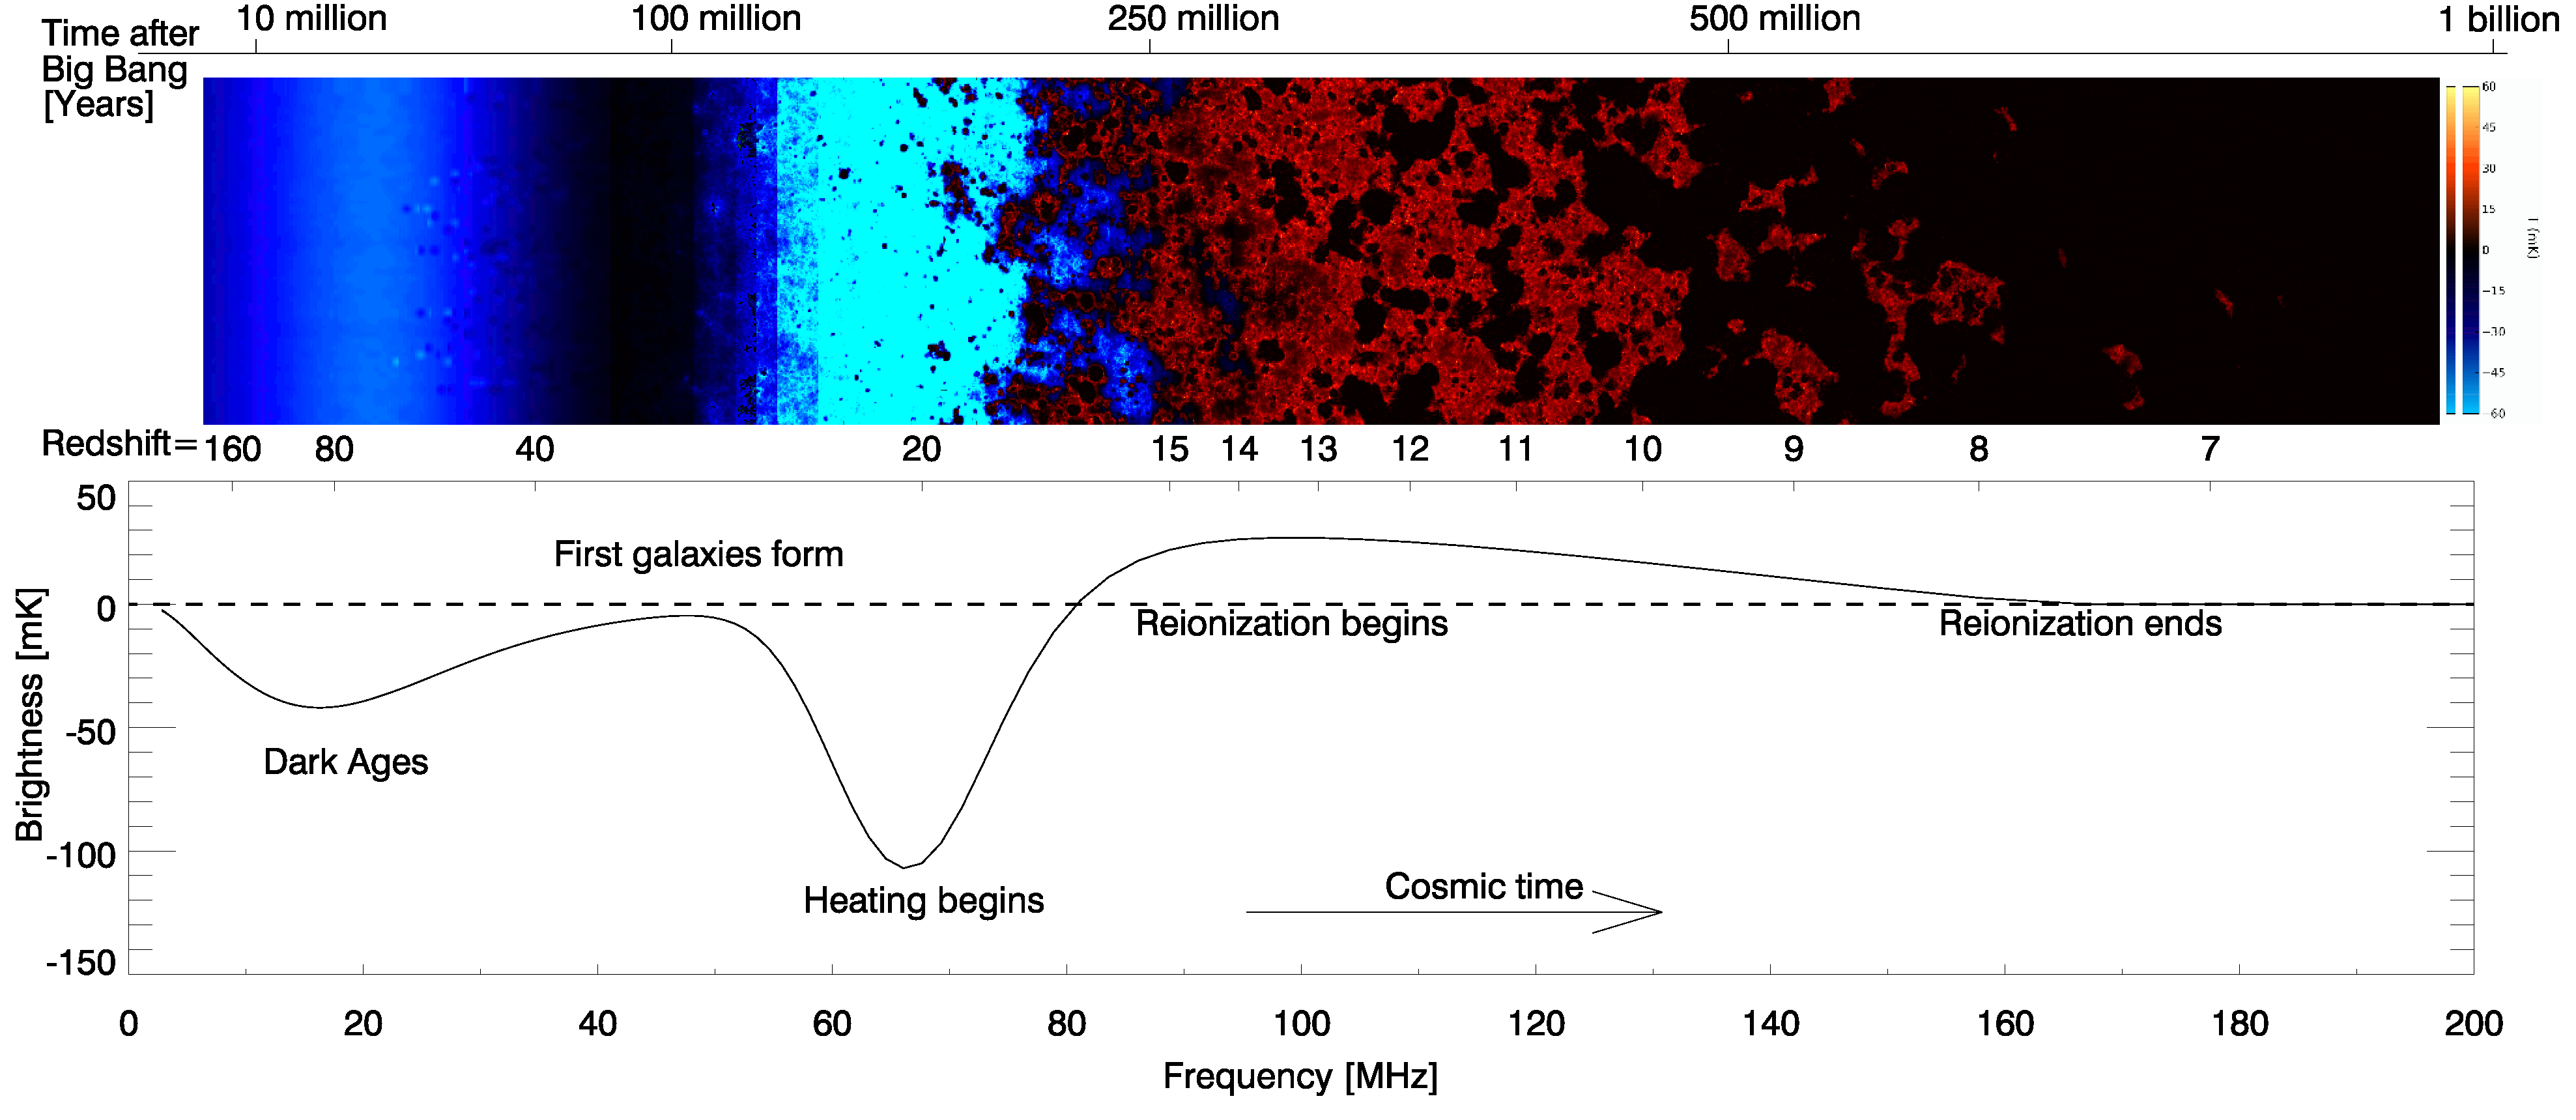
\includegraphics[width=\textwidth]{figures/chapter1/pritchard-2012-global-signal}
    \caption{
        Reproduced from \citet{2012RPPh...75h6901P}.
        get a license to use this figure (hit an error, but email sent (7-7-2018))
    }
    \label{fig:pritchard-global-signal}
\end{figure}

\begin{figure}[t]
    \centering
    \includegraphics[width=\textwidth]{figures/chapter1/history-of-the-universe/history-of-the-universe}
    \caption{
        A radial map of the universe. Known quasars are marked with circles and galaxies are marked
        with stars. The range of comoving distances probed by the OVRO-LWA and HERA are marked with a red
        rectangle and a blue rectangle respectively.
    }
    \label{fig:history-of-the-universe}
\end{figure}

For much of the universe's history, the intergalactic medium (IGM) is ionized or in radiative
equilibrium with the CMB.


\begin{equation}
    T_{21} \approx 27 \left[
        \overbrace{
            x_\text{HI} (1+\delta)
            \left(\frac{\Omega_b h}{0.0327}\right)
        }^{\text{quantity of HI}}
        \left(\frac{\Omega_m}{0.307}\right)^{-1/2}
        \left(\frac{1+z}{10}\right)^{1/2} \linebreak \times
        \overbrace{
            \left(\frac{T_\text{spin} - T_\text{CMB}(z)}{T_\text{spin}}\right)
        }^{\text{relative temperature}}
    \right] \, {\rm mK}
\end{equation}
\citep{2012RPPh...75h6901P}






Given knowledge of the
original wavelength of the photon, and the expansion history of the universe, we can calculate how
long the photon must have been in flight.


Today the CMB is a 2.7~K sea of photons that permeates the universe. This radiation is constantly
cooling due to the inexorable expansion of the universe.


Introduce low frequency telescopes.

Two different types of experiments are currently being designed to target the high-redshift 21~cm
transition:
\begin{enumerate}
    \item single antenna experiments that are attempting to measure the sky-averaged 21~cm signal,
        and
    \item large interferometers that are attempting to measure the three-dimensional spatial power
        spectrum of the 21~cm signal.
\end{enumerate}
Both types require exquisite calibration and roughly five orders of dynamic range against the
blindingly bright foreground radio emission, but are subject to different (but not exclusively
different) systematic instrumental errors.

\begin{figure}[t]
    \centering
    \includegraphics[width=\textwidth]{figures/chapter1/bowman-2018-absorption-trough}
    \caption{
        Reproduced from \citet{2018Natur.555...67B}.
        the Nature thing to get permission for this figure kept redirecting me to a blank page while
        I was trying to fill out the form. Why are all of these things garbage? Still, I need to get
        permission for this figure...
    }
    \label{fig:bowman-absorption-trough}
\end{figure}

\begin{figure}[t]
    \centering
    \includegraphics[width=\textwidth]{figures/chapter1/power-spectrum-upper-limits/power-spectrum-upper-limits}
    \caption{
        Power spectrum amplitude upper limits (95\% confidence) as a function of redshift. The
        shaded region denotes roughly where current theoretical predictions fall.
    }
    \label{fig:power-spectrum-upper-limits}
\end{figure}












\myputbib{thesis}
\end{bibunit}

